\chapter{Memanipulasi File Pada Docker volume}
\section{Pembuka}
Panduan kali ini akan membahas mengenai manipulasi file pada docker volume. Pertama akan membuat dockerfile dengan tambahan konfigurasi WORKDIR.
WORKDIR meupakan sintaks untuk mengarahkan arah direktori kerja /app volume yang akan di mount ke container nanti. File akan dibuat pada direktori ini, Kemudian
user lain akan mengedit, melihat file yang disimpan pada direktori ini.

\section{Langkah memanipulasi file pada docker volume}
    \begin{figure}
    1. Buat dockerfile tambahkan data berikut dan baris WORKDIR "/app"
        \begin{center}
            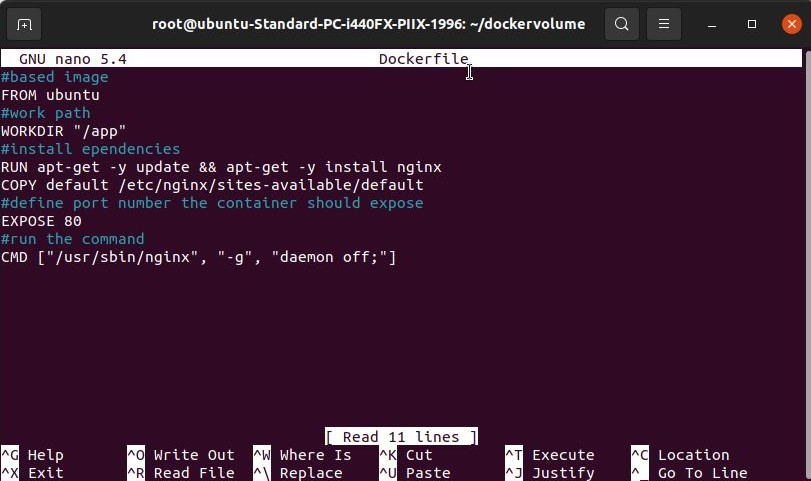
\includegraphics[width=\linewidth]{image/41.jpg}
            \caption{Buat Dockerfile}
            \label{fig:my_figure}
        \end{center}
    
    2. Buat docker images dari Dockerfile yang dibuat tadi
    
    COMMAND: \textcolor{Blue}{docker build .}
        \begin{center}
            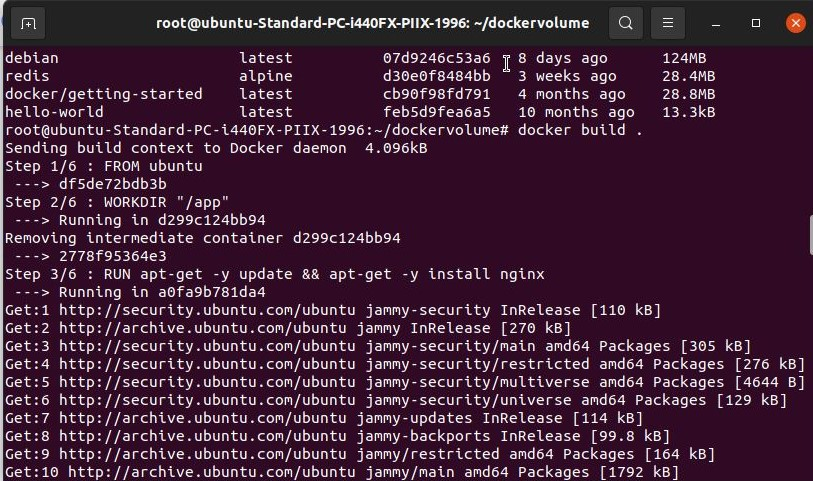
\includegraphics[width=\linewidth]{image/42.jpg}
            \caption{Buat docker images}
            \label{fig:my_figure}
        \end{center}
\end{figure}

\begin{figure}
    3. Beri nama dan tag pada image 
    
    COMMAND: \textcolor{Blue}{docker image tag 006ff0a7b2ea rizkiamel23/web:test678}
    
    Lihat docker images

    COMMAND: \textcolor{Blue}{docker images}
        \begin{center}
            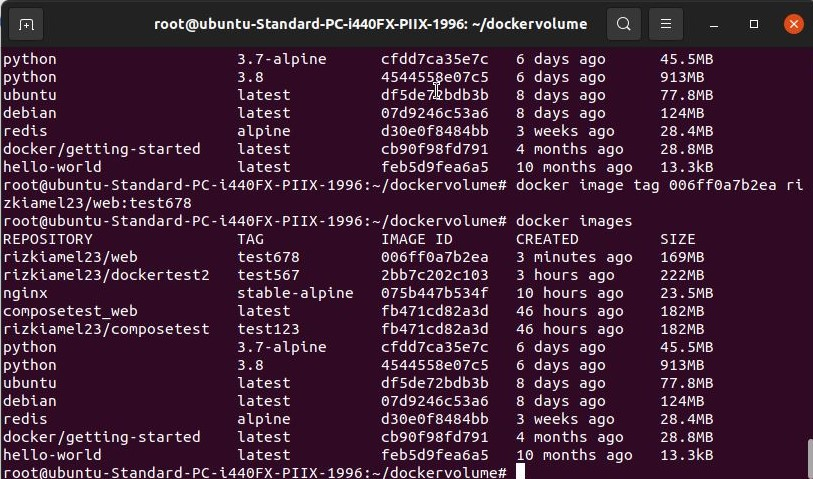
\includegraphics[width=\linewidth]{image/43.jpg}
            \caption{Beri nama dan tag images}
            \label{fig:my_figure}
        \end{center}

    4. Buat volume dengan container, masuk direktori container dan buat file baru

    Buat volume degan container: \textcolor{Gray}{docker run <OPTION> --name <NAMA CONTAINER> -v 
    <NAMA VOLUME:MOUNT DIREKTORI CONTAINER> <NAMA IMAGE:TAG> bash}
    
    COMMAND: \textcolor{Blue}{docker run - -rm -it - -name=web -v volume5:/app rizkiamel23/web:text678 bash}
    
    Setelah masuk bash, buat file baru 
    
    COMMAND: \textcolor{Blue}{cat > index.html}, isi file, Klik CTRL+D
        \begin{center}
            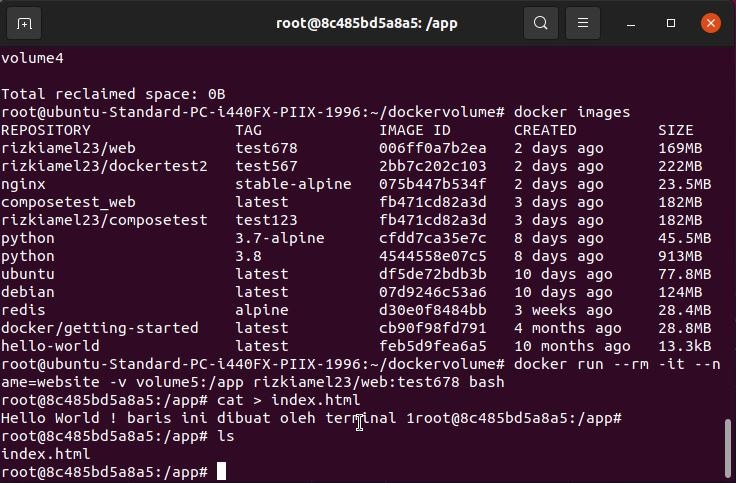
\includegraphics[width=\linewidth]{image/64.jpg}
            \caption{Buat volume, masuk direktori container}
            \label{fig:my_figure}
        \end{center}
\end{figure}

\begin{figure}
    5. Cek file mount
    
    Buka terminal baru :
    
    Klik kanan terminal, new windows 
    
    Masuk akun root :
    
    COMMAND: \textcolor{Blue}{sudo -i}, masukan password root
    
    Cek docker volume :
    
    COMMAND: \textcolor{Blue}{docker ps -a}
    
    Masuk ke direktori container : \textcolor{Gray}{docker exec -t -i <ID CONTAINER> /bin/bash}
    
    COMMAND: \textcolor{Blue}{docker exec -t -i 8c485bd5a8a5 /bin/bash}
    
    Lihat list file :
    
    COMMAND: \textcolor{Blue}{ls}
    
    Lihat isi file index.html :
    
    COMMAND: \textcolor{Blue}{cat index.html}
        \begin{center}
            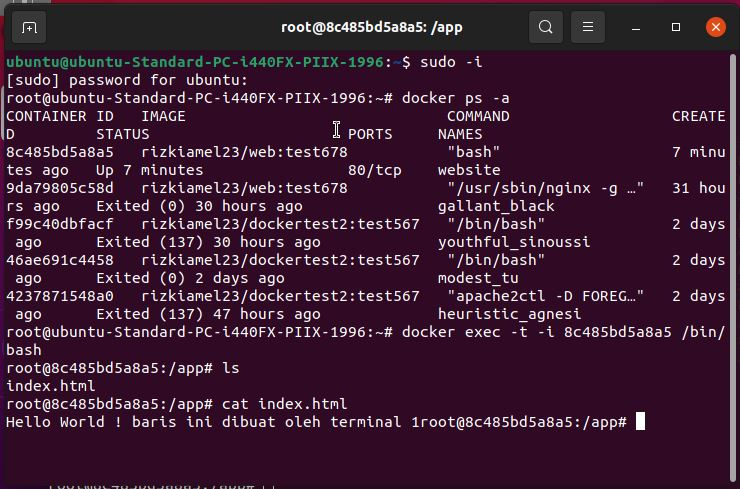
\includegraphics[width=\linewidth]{image/65.jpg}
            \caption{Cek file mount}
            \label{fig:my_figure}
        \end{center}
\end{figure}

\begin{figure}
    6. Lakukan inspect volume 
    
    Keluar dari mode bash :
    
    COMMAND: \textcolor{Blue}{exit}
    
    Lihat list volume :
    
    COMMAND: \textcolor{Blue}{docker volume ls}
    
    Inspect volume : \textcolor{Gray}{docker volume inspect <NAMA VOLUME>}
    
    COMMAND: \textcolor{Blue}{docker volume inspect volume5}
        \begin{center}
            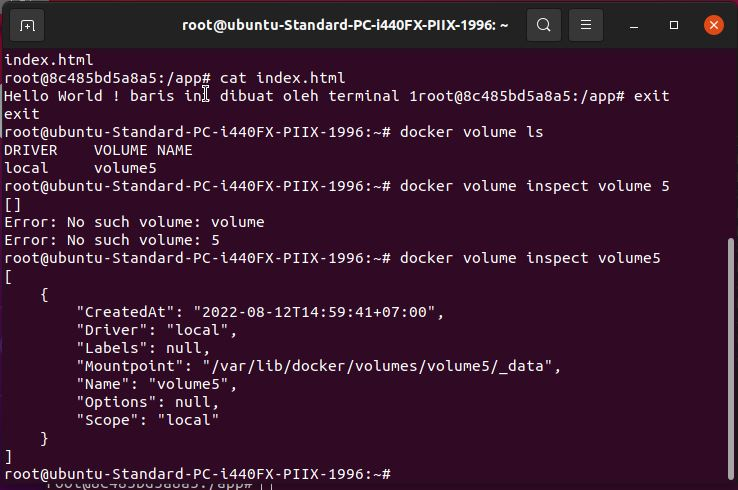
\includegraphics[width=\linewidth]{image/66.jpg}
            \caption{Inspect volume}
            \label{fig:my_figure}
        \end{center}

    Dari gambar diatas dapat dilihat path direktori yang di mounted oleh volume, path ini merupakan
    tempat penyimpanan pada volume. walaupun container dihapus selama volumnya tidak dihapus 
    direktori ini tetap ada, direktori ini dapat dihapus jika volumenya dihapus.
\end{figure}

\begin{figure}
    7. Masuk direktori mount volume
    
    Masuk direktori mount volume : \textcolor{Gray}{cd <PATH DIREKTORI MOUNT>}
    
    COMMAND: \textcolor{Blue}{cd /var/lib/docker/volumes/volume5/data}
    
    Lihat list file :
    
    COMMAND: \textcolor{Blue}{ls}
    
    Edit file :
    
    COMMAND: \textcolor{Blue}{nono index.html}
        \begin{center}
            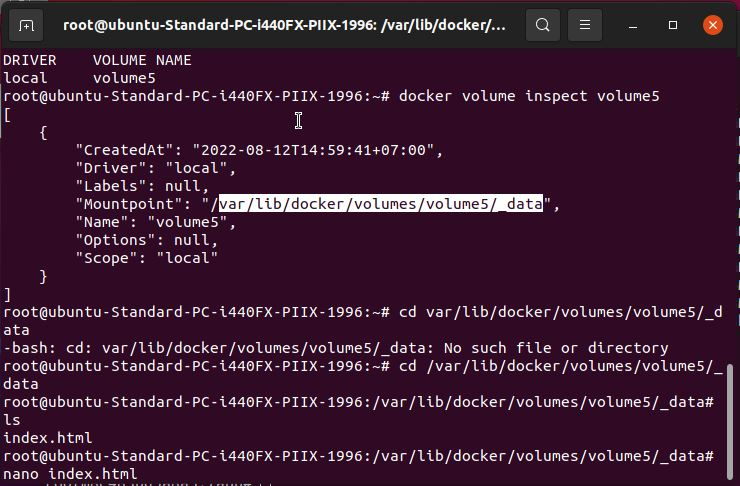
\includegraphics[width=\linewidth]{image/67.jpg}
            \caption{Edit file}
            \label{fig:my_figure}
        \end{center}

    Kemudian lakukan edit file lalu tekan CTRL+X, Y, ENTER
        \begin{center}
            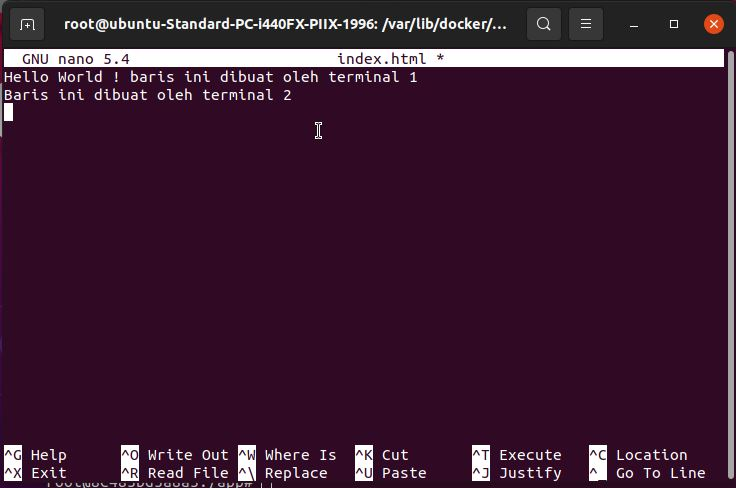
\includegraphics[width=\linewidth]{image/68.jpg}
            \caption{Edit file dan simpan}
            \label{fig:my_figure}
        \end{center}
\end{figure}

\begin{figure}
    8. Buka terminal sebelumnya, cek isi file

    Cek isi file :

    COMMAND: \textcolor{Blue}{cat index.html}
        \begin{center}
            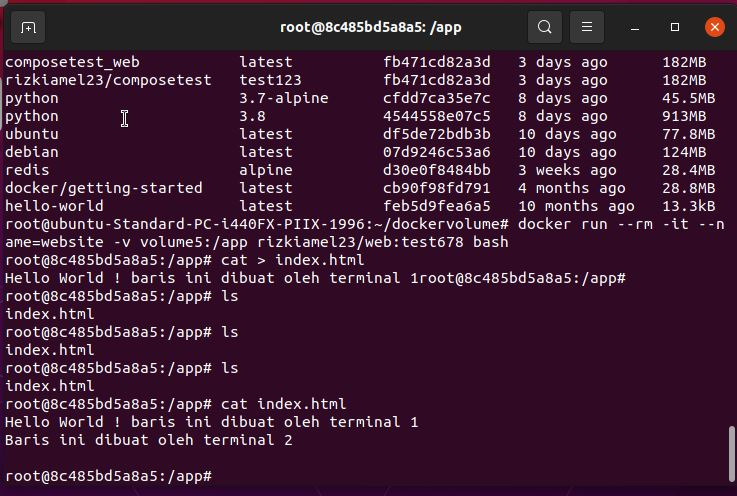
\includegraphics[width=\linewidth]{image/70.jpg}
            \caption{Cek isi file}
            \label{fig:my_figure}
        \end{center}
    
    Dari gambar diatas file bisa dimodifikasi selama volume belum dihapus 
\end{figure}

